% Copyright (C)  2018  TANSORIER.
% Permission is granted to copy, distribute and/or modify this document
% under the terms of the GNU Free Documentation License, Version 1.3
% or any later version published by the Free Software Foundation;
% with no Invariant Sections, no Front-Cover Texts, and no Back-Cover Texts.
% A copy of the license is included in the section entitled "GNU
% Free Documentation License".

% https://www.gnu.org/licenses/fdl-1.3.html

% compress option to have horyzontal circle
\documentclass[compress]{beamer}

%%%%%%%%%%%%%%%%%%%%%%%%%%%%%%%%%%%%%%%%%%%%%%%%%%%%%%%%%%%%%%%%%%%%%

% Thèmes suppélmentaires
\useoutertheme[]{miniframes} % barre menu du haut
\setbeamertemplate{frametitle}[default] % replace le titre à la bonne place
\useinnertheme{rounded} % arrondi les angles

\setbeamertemplate{footline}[text line]{
\textcolor{gray}{%
	\parbox{\linewidth}{\vspace*{-8pt}Smile ECS\hfill\insertshortauthor\hfill\insertpagenumber/\inserttotalframenumber}}
}
\beamertemplatenavigationsymbolsempty

% Language
\usepackage[french]{babel}
\usepackage[utf8]{inputenc}
\usepackage[T1]{fontenc}

% Display Table Of Content spécific for smilebeamer
% Force to get empty
\AtBeginSection[]{}
\AtBeginSubsection[]{}
%{
%  \begin{frame}<beamer>
%  \frametitle{Plan}
%  \tableofcontents[currentsection]
%  \end{frame}
%}

% Change color of definiton block
\AtBeginEnvironment{definition}{%
	\setbeamercolor{block title}{use=example text,fg=example text.fg,bg=example text.fg!20!bg}
	\setbeamercolor{block body}{parent=normal text,use=block title,bg=block title.bg!50!bg}
}

% caption size reduce
\usepackage{caption}
\setbeamerfont{caption}{size=\scriptsize}

% code coloration
\usepackage{listings}
% L'option "[fragile]" doit être rajouté au frame pour pouvoir utiliser correctement
% la police verbatim
\usepackage{color}
\lstset{
  breaklines=true,
  tabsize=4,
  backgroundcolor=\color[RGB]{49,54,59},
  basicstyle=\footnotesize\ttfamily\color{white},
  commentstyle=\itshape\color[RGB]{0,136,136},
  morecomment=[l]{\#},
  morekeywords={*,\$,\{,\}},
  stringstyle=\itshape\color[RGB]{218,116,0},
  showstringspaces=false,
  frame=LTBR,
}
\lstdefinestyle{shell}{
  basicstyle=\fontsize{7pt}{7pt}\ttfamily\color{white},
  language=bash,
  keywords={\$},
  keywordstyle=\bfseries\color[RGB]{66,198,66},
  literate=
    {├}{{\smash{\raisebox{-1ex}{\rule{1pt}{\baselineskip}}}\raisebox{0.5ex}{\rule{1ex}{1pt}}}}1 
    {─}{{\raisebox{0.5ex}{\rule{1.5ex}{1pt}}}}1 
    {│}{{\smash{\raisebox{-1ex}{\rule{1pt}{\baselineskip}}}\raisebox{0.5ex}{\rule{1ex}{0pt}}}}1 
    {└}{{\smash{\raisebox{0.5ex}{\rule{1pt}{\dimexpr\baselineskip-1.5ex}}}\raisebox{0.5ex}{\rule{1ex}{1pt}}}}1
}
\lstdefinestyle{bitbake}{
  language=bash,
  alsoletter=-,
  morekeywords={\$,\{,\}},
  morekeywords={BBFILES,BBFILE_COLLECTIONS,BBFILE_PATTERN_meetup,BBFILE_PRIORITY_meetup,%
  BBLAYERS,MACHINE,DISTRO,LAYERDEPENDS_meta-python,DISTRO_FEATURES_remove,%
  DISTRO_FEATURES_append,VIRTUAL-RUNTIME_init_manager,require,DISTRO_NAME,%
  DISTRO_VERSION,DISTRO_FEATURES_DEFAULT,DISTRO_FEATURES_LIBC,PACKAGE_CLASSES,%
  POKY_DEFAULT_DISTRO_FEATURES,DISTRO_FEATURES,IMAGE_FEATURES,IMAGE_INSTALL,BBPATH},
  keywordstyle=\bfseries\color[RGB]{152,251,152},
}

% pour les schemas
\usepackage{tikz}
\usepackage{tikz}

% Pour utiliser des colonnes
\usepackage{multicol}

%%%%%%%%%%%%%%%%%%%%%%%%%%%%%%%%%%%%%%%%%%%%%%%%%%%%%%%%%%%%%%%%%%%%%
\title[Yocto]{Yocto - \texttt{devtool} - et autres… \\ \textbf{Comment développer efficacement sous Yocto}}

\author[Mickaël Tansorier]{Mickaël Tansorier}

\date[Mars 2018]{Présentation des outils et commandes pratique pour travailler sous Yocto}
%%%%%%%%%%%%%%%%%%%%%%%%%%%%%%%%%%%%%%%%%%%%%%%%%%%%%%%%%%%%%%%%%%%%%

\begin{document}
%\tableofcontents[subsectionstyle=hide]

% *******************************
% ****     PAGE DE GARDE     ****
% *******************************

\begin{frame}
\titlepage
\end{frame}


% *******************************
% ****      INTRODUCTION     ****
% *******************************

\begin{frame}
\underline{Objectif de la présentation}
\begin{itemize}
	\item Présenter rapidement Yocto
	\item Présenter des outils utiles
	\begin{itemize}
		\item \texttt{devtool}
		\item \texttt{opkg}
		\item \texttt{…}
	\end{itemize}
\end{itemize}
\end{frame}


\begin{frame}{Plan}
\tableofcontents[hideallsubsections]
\end{frame}

% *******************************
% ****     PRÉSENTATION      ****
% *******************************
\section{Présentation rapide de Yocto}

\begin{frame}{Présentation de Yocto}
\tableofcontents[currentsection,hideallsubsections]
\end{frame}

\begin{frame}{Présentation de Yocto}
\begin{center}

\includegraphics[width=0.7\textwidth]{logos/yocto-project-transp.png}
\end{center}
\end{frame}

\begin{frame}{D'où vient ce nom ?}
\begin{definition}
	Yocto est un préfixe représentant 10\textsuperscript{-24} unités (SI)
\end{definition}
\end{frame}

\begin{frame}
\begin{block}{Qu'est ce qu'est vraiment Yocto ?}
	Yocto est un outil qui répond au besoin de générer une distribution
	\textbf{Linux embarqué} pour un matériel \textbf{dédié}.
\end{block}
\end{frame}

\begin{frame}
Yocto utilise le principe de \texttt{MACHINE} et de \texttt{DISTRO} qui sent à la différenciation de l’\textbf{architecture matérielle} de l’\textbf{application logicielle} de la cible
\begin{itemize}
	\item \texttt{MACHINE} : définit l’architecture matérielle
	\item \texttt{DISTRO} : définit la distribution à générer
\end{itemize}
Il dispose de plusieurs outils très pratique pour le développement:
\begin{itemize}
	\item \texttt{devtool}
	\item \texttt{ipk}/\texttt{opkg}
\end{itemize}
\end{frame}

\begin{frame}
\tikzstyle{recette} = [draw, fill=orange!70, rectangle, minimum height=2.5em, minimum width=10em,rounded corners=5pt]
\tikzstyle{cadre} = [rectangle, draw, minimum height=12em, minimum width=8.5em, fill=orange!70]
\begin{center}
\begin{tikzpicture}[node distance=1.2cm]
% Yocto
\node[draw,rectangle,minimum height=8cm, minimum width=10cm, fill=orange!70, label={[anchor=north]north:Yocto}] (YOCTO) {};
% Bitbake
\node[draw,rectangle, minimum height=2.5em, minimum width=8cm,rounded corners=5pt, fill=blue!40, yshift=2.8cm] (bitbake) {BITBAKE};
% Layers
\node[draw,rectangle, minimum height=2.5cm, minimum width=3cm,rounded corners=5pt, fill=green!70!black!70, yshift=0.7cm, xshift=-2cm, label={[anchor=north]north:LAYER A}] (layer-A) {};
\node[draw,rectangle, right of=layer-A, minimum height=2.5cm, minimum width=3cm,rounded corners=5pt, fill=green!70!black!70, xshift=2.6cm, label={[anchor=north]north:LAYER B}] (layer-B) {};
\node[draw,rectangle, below of=layer-A, minimum height=2.5cm, minimum width=3cm,rounded corners=5pt, fill=green!70!black!70, yshift=-1.8cm, label={[anchor=north]north:LAYER C}] (layer-C) {};
\node[draw,rectangle, below of=layer-B, minimum height=2.5cm, minimum width=3cm,rounded corners=5pt, fill=green!70!black!70, yshift=-1.8cm, label={[anchor=north]north:LAYER D}] (layer-D) {};
% Recettes
\node[draw,rectangle, below of=layer-A, fill=red!80!black!70, xshift=0cm, yshift=1.6cm] (rectte-A1) {RECETTE A1};
\node[draw,rectangle, below of=rectte-A1, fill=red!80!black!70, yshift=0.6cm] (rectte-A2) {RECETTE A2};
\node[draw,rectangle, below of=rectte-A2, fill=red!80!black!70, yshift=0.6cm] (rectte-A3) {RECETTE A3};
\node[draw,rectangle, below of=layer-B, fill=red!80!black!70, xshift=0cm, yshift=1.6cm] (rectte-B1) {RECETTE B1};
\node[draw,rectangle, below of=rectte-B1, fill=red!80!black!70, yshift=0.6cm] (rectte-B2) {RECETTE B2};
\node[draw,rectangle, below of=rectte-B2, fill=red!80!black!70, yshift=0.6cm] (rectte-B3) {RECETTE B3};
\node[draw,rectangle, below of=layer-C, fill=red!80!black!70, xshift=0cm, yshift=1.6cm] (rectte-C1) {RECETTE C1};
\node[draw,rectangle, below of=rectte-C1, fill=red!80!black!70, yshift=0.6cm] (rectte-C2) {RECETTE C2};
\node[draw,rectangle, below of=rectte-C2, fill=red!80!black!70, yshift=0.6cm] (rectte-C3) {RECETTE C3};
\node[draw,rectangle, below of=layer-D, fill=red!80!black!70, xshift=0cm, yshift=1.6cm] (rectte-D1) {RECETTE D1};
\node[draw,rectangle, below of=rectte-D1, fill=red!80!black!70, yshift=0.6cm] (rectte-D2) {RECETTE D2};
\node[draw,rectangle, below of=rectte-D2, fill=red!80!black!70, yshift=0.6cm] (rectte-D3) {RECETTE D3};
\end{tikzpicture}
\end{center}
\end{frame}


%
% ****     LE COEUR      ****
%
\subsection{Le coeur}

\begin{frame}
\begin{center}
\textcolor{orange}{\huge{Avant de passer aux recettes, qui fait le travail dans Yocto ?}}
\end{center}
\end{frame}

\begin{frame}{bitbake}
\begin{block}{bitbake c'est quoi ?}
\begin{itemize}
	\item Un moteur d'exécution de tâches écrite en Python
	\item Fonctionne en ligne de commande
	\item Exécute automatiquement les tâches nécessaires à la fabrication de la cible fournie
\end{itemize}
\end{block}
\end{frame}


\begin{frame}{bitbake}
\tikzstyle{block} = [draw, fill=orange!70, rectangle, minimum height=2.5em, minimum width=10em,rounded corners=5pt]
\tikzstyle{arrow} = [thick,->,>=stealth]
\begin{center}
\begin{tikzpicture}[node distance=1.2cm]
\node [block, fill=green!60!black!50]   (read)   {LECTURE RECETTE};
\node [block, below of=read]  (fetch)  {FETCH};
\node [block, below of=fetch] (unpack) {UNPACK};
\node [block, below of=unpack] (patch) {PATCH};
\node [block, below of=patch] (configure) {CONFIGURE};
\node [block, right of=configure, xshift=3cm] (compile) {COMPILE};
\node [block, above of=compile] (install) {INSTALL};
\node [block, above of=install] (package) {PACKAGE};
\node [block, above of=package, fill=green!60!black!50] (rootfs) {ROOFS};

\draw[arrow] (read) -- (fetch);
\draw[arrow] (fetch) -- (unpack);
\draw[arrow] (unpack) -- (patch);
\draw[arrow] (patch) -- (configure);
\draw[arrow] (configure) -- (compile);
\draw[arrow] (compile) -- (install);
\draw[arrow] (install) -- (package);
\draw[arrow] (package) -- (rootfs);
\end{tikzpicture}
\end{center}
\textcolor{gray}{\tiny{Pour avoir les vrais étapes d'une recette: \texttt{bitbake <recette> -c listtasks}}}
\end{frame}

\subsection{recette}

\begin{frame}{recette}
\begin{block}{À quoi ça ressemble une recette ?}
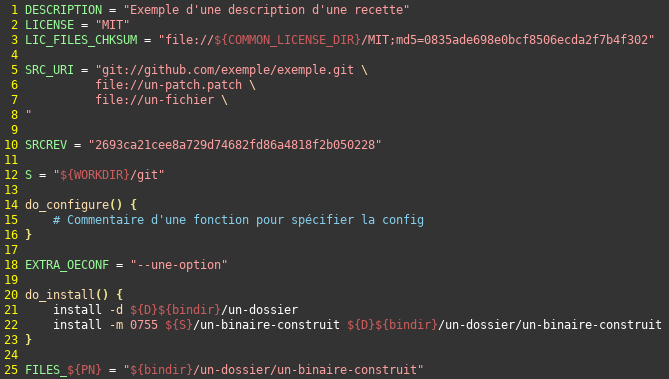
\includegraphics[width=\textwidth]{images/recette-yocto.png}
\end{block}
\end{frame}



% *******************************
% ****    OUTILS DEVTOOL    ****
% *******************************
\section{\texttt{devtool}}

\begin{frame}{\texttt{devtool}}
\tableofcontents[currentsection,hideallsubsections]
\end{frame}

\begin{frame}{\texttt{devtool}}
\begin{center}
\textcolor{orange}{\huge{Exemple de l'utilisation de l'outil \texttt{devtool}}}
\end{center}
\end{frame}

\subsection{Les commandes de base}

\begin{frame}
\texttt{devtool} est un outils très utiles lorsque l'on souhaite créer, développer ou modifier une recette et ses sources.\newline
\newline
Les commandes de base:
\begin{description}
	\item[\texttt{devtool add}] Ajoute un nouveau software à construire
	\item[\texttt{devtool modify}] Génère un environnement pour modifier les sources d'une recette
	\item[\texttt{devtool upgrade}] Met à jour une recette existante
	\item[\texttt{devtool reset}] Arrête le contexte de développement
\end{description}
\end{frame}

\begin{frame}
Les sources peuvent provenir de plusieurs endroits différent
\begin{center}
	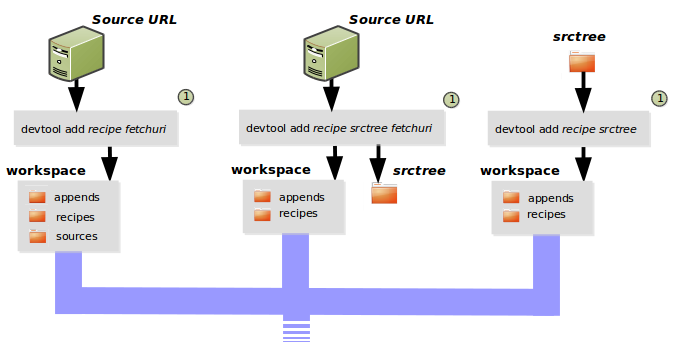
\includegraphics[width=1\textwidth]{images/devtool-add-src.png}
\end{center}
\end{frame}

\begin{frame}
De même pour modifier une recette
\begin{center}
	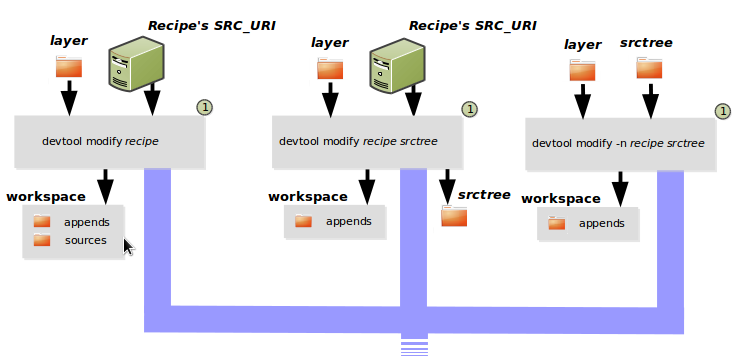
\includegraphics[width=1\textwidth]{images/devtool-modify-src.png}
\end{center}
\end{frame}

\subsection{Le comportement de \texttt{devtool}}

\begin{frame}[fragile]
Dès lors \texttt{devtool} créer un layer spécial (\texttt{workspace}) qui prend la priorité maximal sur les autres layers.
\begin{lstlisting}[style=shell,breaklines=false,xleftmargin=-16px,xrightmargin=-16px]
$ bitbake-layers show-layers
NOTE: Starting bitbake server...
layer              path                                      priority
=========================================================================
meta               /home/[...]/meta                          5
meta-poky          /home/[...]/meta-poky                     5
meta-yocto-bsp     /home/[...]/meta-yocto-bsp                5
workspace          /home/[...]/build/workspace               99
meta-raspberrypi   /home/[...]/build/../meta-raspberrypi     9
meta-python        /home/[...]/build/../meta-openembedded/meta-python  7
meta-oe            /home/[...]/build/../meta-openembedded/meta-oe  6
meta-meetup        /home/[...]/build/../meta-meetup           10
\end{lstlisting}
\end{frame}

\begin{frame}[fragile]
Dans ce layer on retrouve
\begin{itemize}
	\item les sources mis sous git et patché
	\item un bbappend de la recette
\end{itemize}
\begin{lstlisting}[style=shell]
$ cd $POKY/build/workspace/
$ tree -L 2 
.
├── appends
│   └── weston_2.0.0.bbappend
├── conf
│   └── layer.conf
├── README
└── sources
    └── weston
\end{lstlisting}
\end{frame}

\subsection{Exemple pratique}

\begin{frame}
\begin{center}
\textcolor{orange}{\huge{Exemple pratique avec la recette \texttt{weston}}}
\end{center}
\end{frame}

\begin{frame}[fragile]
Modification avec \texttt{devtool} des sources de weston
\begin{lstlisting}[style=shell]
$ devtool modify weston
$ cd $POKY/build/workspace/sources/weston/
$ vim libweston/compositor-wayland.c +1655
\end{lstlisting}

Ajout du patch "Fix an uninitialized variable"
% https://github.com/wayland-project/weston/commit/6b2fb180d99bb9d6deaddb1cdf735422d4dd5b93
\begin{lstlisting}[escapeinside={<@}{@>}]
@@ -1652,6 +1652,7 @@ input_handle_axis(void *data, struct wl_pointer *pointer,
 
 	weston_event.axis = axis;
 	weston_event.value = wl_fixed_to_double(value);
<@\textcolor{green!80!black}{\texttt{+\,\,\,\, weston\_event.has\_discrete = false;}}@>
 
 	if (axis == WL_POINTER_AXIS_VERTICAL_SCROLL &&
 	    input->vert.has_discrete) {
\end{lstlisting}
\end{frame}

\begin{frame}[fragile]
Les étapes:
\begin{enumerate}
\item Faire la modification
\item Tester normalement
\item Commiter
\item Appliquer la modification sous forme de patch
\begin{lstlisting}[style=shell]
$ devtool update-recipe weston
[...]
NOTE: Adding new patch 0001-Fix-an-uninitialized-variable.patch
NOTE: Updating recipe weston_2.0.0.bb
\end{lstlisting}
\item Ajouter la modification dans son layer
	% L'ajout d'un bbappend dans meta-meetup
	% Supprimer l'ajout de meta/recipes-graphics/wayland/weston_2.0.0.bb
	% Le déplacement du patch dans meta-meetup
\item Arrêter devtool
\begin{lstlisting}[style=shell]
$ devtool reset weston
\end{lstlisting}
\end{enumerate}
\end{frame}

\begin{frame}[fragile]
Dans le cas où vous modifiez déjà une recette avec un bbappend, je vous conseil d'extraire les patchs à la main:
\begin{lstlisting}[style=shell]
$ cd $POKY/build/workspace/sources/weston/
$ git format patch -<nb_patch>
\end{lstlisting}
Il ne reste plus qu'a copier ces patch dans la recette et d'ajouter dans le bbappend avec:
\begin{lstlisting}[style=shell]
FILESEXTRAPATHS_prepend := "${THISDIR}/${PN}:"
SRC_URI += "file://000X-mon-patch.patch"
\end{lstlisting}
\end{frame}

\subsection{Déployer directement vos modifications sur cible}

\begin{frame}
\begin{center}
\textcolor{orange}{\huge{Exemple pour deployer directement ses modifications sur cible}}
\end{center}
\end{frame}

\begin{frame}[fragile]
Après modification de source avec devtool il est possible de déployer ces modification directement sur une cible avec:
\begin{lstlisting}[style=shell]
$ devtool deploy-target <recette> <user@cible>
\end{lstlisting}
La cible doit disposer d'un serveur ssh. \newline
\newline
Attention, devtool n'envoit pas un paquet mais le résultat de la recette, donc pas besoin d'un \texttt{package-management} sur cible.\\
Une fois votre mise au point terminée vous pouvez supprimer tous les fichiers ajoutés par votre recette la commande:
\begin{lstlisting}[style=shell]
$ devtool undeploy-target <recette> <user@cible>
\end{lstlisting}
\end{frame}


% *******************************
% ****    OUTILS OPKG et IPK   ****
% *******************************
\section{\texttt{opkg} et \texttt{ipk}}

\begin{frame}
\tableofcontents[currentsection,hideallsubsections]
\end{frame}

\begin{frame}
\begin{center}
\textcolor{orange}{\huge{Exemple de l'utilisation des l'outils \texttt{opkg} et \texttt{ipk}}}
\end{center}
\end{frame}

\subsection{\texttt{opkg} un gestionnaire de paquets}

\begin{frame}{\texttt{opkg} est un gestionnaire de paquets}
\texttt{opkg} est gestionnaire de paquet tout comme apt l'est pour les distribution hérité de Debian.\newline
\newline
Les commandes de base:
\begin{description}
	\item[\texttt{opkg update}] Mettre à jour la list des paquets
	\item[\texttt{opkg upgrade <pkgs>}] Mettre à jour un paquet
	\item[\texttt{opkg install <pkgs|url>}] Installer un paquet
	\item[\texttt{opkg remove <pkgs>}] Supprimer un paquet
\end{description}
\end{frame}

\subsection{Créer son propre serveur de paquet}

\begin{frame}[fragile]{Créer son propre serveur \texttt{opkg}}
Pour créer son serveur opkg il suffit d'avoir un sereur http.\newline
On peut le crée simplement avec python en remplaçant les variable par leur valeur :
\begin{lstlisting}[style=shell]
$ cd ${POKY}/build/tmp/deploy/ipk
$ ${NATIVE_SDK_BINS}/usr/bin/python-native/python -m SimpleHTTPServer ${IPK_SERVER_PORT}
\end{lstlisting}
Avec python3:
\begin{lstlisting}[style=shell]
$ cd ${POKY}/build/tmp/deploy/ipk
$ ${NATIVE_SDK_BINS}/usr/bin/python-native/python3 -m http.server ${IPK_SERVER_PORT}
\end{lstlisting}
\end{frame}

\begin{frame}[fragile]{Définir le serveur \texttt{opkg} sur cible}
Ajouter ces lignes dans le fichier \texttt{opkg.conf} en remplaçant les variable correspondante par leur valeur:
\begin{lstlisting}[style=shell,xleftmargin=-18px,xrightmargin=-18px]
src/gz all http://ipk-server:${IPK_SERVER_PORT}/all
src/gz ${MACHINE_ARCH} http://ipk-server:${IPK_SERVER_PORT}/${MACHINE_ARCH} 
src/gz ${MACHINE_SOCARCH} http://ipk-server:${IPK_SERVER_PORT}/${MACHINE_SOCARCH}
src/gz ${TUNE_PKGARCH} http://ipk-server:${IPK_SERVER_PORT}/${TUNE_PKGARCH}
\end{lstlisting}
\textcolor{gray}{\tiny{Recette opkg}}
\newline
Ajouter dans \texttt{/etc/hosts} le serveur:
\begin{lstlisting}[style=shell]
${IP_HOST}     ipk-server
\end{lstlisting}
\textcolor{gray}{\tiny{Recette netbase}}
\end{frame}


% *******************************
% ****    OUTILS DIVERS   ****
% *******************************
\section{Outils et commandes diverses}

\begin{frame}
\tableofcontents[currentsection,hideallsubsections]
\end{frame}

\begin{frame}
\begin{center}
\textcolor{orange}{\huge{Quelques outils et commandes diverses qui peuvent intéresser}}
\end{center}
\end{frame}

\subsection{La plus puissante option}

\begin{frame}[fragile]{environnement}
Pour connaitre l'état de n'importe quelle recette et quelle variable est compléter par quel fichier de recette, l'option \texttt{-e} est le plus puissant.\newline
\begin{lstlisting}[style=shell]
$ bitbake <recipe> -e
\end{lstlisting}
La sortie est assez velue, il vaut mieux l'ouvrir dans un éditeur comme:
\begin{lstlisting}[style=shell]
$ bitbake <recipe> -e | vim -
\end{lstlisting}
\end{frame}

\subsection{devshell}

\begin{frame}[fragile]{environnement}
Si vous souhaitez tester des commandes dans un environnement de cross compilation, l'option \texttt{devshell} est l'outils qu'il faut:
\begin{lstlisting}[style=shell]
$ bitbake <recipe> -c devshell
\end{lstlisting}
\end{frame}

\subsection{defconfig}

\begin{frame}[fragile]{defconfig}
Ajouter un fichier de configuration.\newline
\newline
Pour la plupart des paquets la gestion de yocto reconnais les defconfig. Il faut ajouter dans un bbappend pour dans une recette maitrisé:
\begin{lstlisting}[style=shell]
FILESEXTRAPATHS:prepend := "${THISDIR}/${PN}:"
SRC_URI += "file://defconfig"
\end{lstlisting}
\end{frame}

\begin{frame}[fragile]{savedefconfig}
Ajouter une option de configuration à un paquet facilement.\newline
\newline
Ceci fonctionne si vous avez le defconfig dans votre layer.
\begin{enumerate}
\item Ajouter une config
\begin{lstlisting}[style=shell]
$ bitbake linux-fslc -c menuconfig
\end{lstlisting}
\item Tester
\item Générer le nouveau defconfig
\begin{lstlisting}[style=shell]
$ bitbake linux-fslc -c savedefconfig
\end{lstlisting}
\item Remplacer le defconfig par sa génération
\end{enumerate}
\end{frame}

\begin{frame}[fragile]{diffconfig}
Ajouter une option de configuration à un paquet facilement.
\begin{enumerate}
\item Ajouter une config
\begin{lstlisting}[style=shell]
$ bitbake linux-fslc -c menuconfig
\end{lstlisting}
\item Tester
\item Extraire la configuration et ses dépendances mutualisé
\begin{lstlisting}[style=shell]
$ bitbake linux-fslc -c diffconfig
linux-fslc-4.10-r0 do_diffconfig: Config fragment has been dumped into:
 /home/user/yocto/build/tmp/work/archi/linux-fslc/4.10-r0/fragment.cfg
\end{lstlisting}
\item Ajouter le fragment à la recette
\begin{lstlisting}[style=shell]
FILESEXTRAPATHS_prepend := "${THISDIR}/${PN}:"
SRC_URI += "file://myfragment.cfg"
\end{lstlisting}
\textcolor{gray}{\tiny{Après la génération du diffconfig il faut ajouter l'option à la recette car elle est retiré du config}}
\end{enumerate}
\end{frame}

\subsection{Compiler le plus loin possible}

\begin{frame}[fragile]{Compilation}
Si vous souhaitez compiler une image le plus loin possible après une erreur:
\begin{lstlisting}[style=shell]
$ bitbake <image> -k
\end{lstlisting}
\end{frame}

\subsection{oe-pkgdata-util}

\begin{frame}[fragile]{Quel parquet embarque quoi comme ficher}
Lister les fichier contenue dans un paquet:
\begin{lstlisting}[style=shell]
$ oe-pkgdata-util list-pkg-files <recipe>
\end{lstlisting}
Trouver quel paquet fournis quel fichier:
\begin{lstlisting}[style=shell]
$ oe-pkgdata-util find-path /etc/opkg/pokg.conf
\end{lstlisting}
\end{frame}

\subsection{buildhistory}

\begin{frame}[fragile]{buildhistory}
Buildhistory fourni un ensemble de détails sur le contenue des paquets, leur dépendances, et leur inclusion dans une image.\newline
\newline
Ajouter dans \texttt{conf/local.conf}:
\begin{lstlisting}[style=shell]
INHERIT += "buildhistory"
BUILDHISTORY_COMMIT = "1"
\end{lstlisting}
Le résultat se situe dans le dossier de build dans \texttt{buildhistory}.
\end{frame}

\subsection{autocompletion}

\begin{frame}[fragile]{Autocompletion}
Pour faciliter le développement l'autocompletion est plus confortable.\newline
\newline
Il existe des projets, mais qui date un peut...
\url{https://github.com/sergioprado/bitbake-bash-completion}
\url{https://github.com/lukaszgard/bitbake-completion}\newline
\newline
Il faut copier les fichier dans:
\begin{lstlisting}[style=shell]
/etc/bash_completion.d/
\end{lstlisting}
Suivez les instructions des dépôts.
\end{frame}


% *******************************
% ****     CONCLUSION    ****
% *******************************
\section*{Questions}

\begin{frame}{Sources}
Ce document à été rédigé à partir des sources suivantes:\newline
\begin{itemize}
	\item \url{www.yoctoproject.org}
	\item \url{www.linuxembedded.fr}
	\item \url{https://openwrt.org/docs/guide-user/additional-software/opkg}
\end{itemize}
\end{frame}

\begin{frame}
\centering
\textcolor{orange}{\huge{Merci de votre attention !}}

\textcolor[RGB]{99,153,253}{Quetions ?}


\includegraphics[width=0.5\textwidth]{logos/smile-logo.png}

Mickaël Tansorier

\url{mickael.tansorier@smile.fr}

\url{mickael@tansorier.fr}

\vfill
\textcolor{gray}{\tiny{GNU Free Documentation License, Version 1.3}}
\end{frame}

\end{document}
